\documentclass{beamer}

%--------------------------------------------------------------

\usepackage[latin1]{inputenc}
\usepackage[T1]{fontenc}
\usepackage{tikz}
\usetikzlibrary{shadows.blur}
\usetikzlibrary{shapes.symbols}

\usetheme{Madrid}
\usecolortheme{beaver}

\graphicspath{{img/}}

%--------------------------------------------------------------

\title[Visualizzazione di Algoritmi in HTML5]{Visualizzazione grafica di Algoritmi in HTML5}
\author{Tommaso~Papini}
\institute[UniFI]{
	Universit� degli Studi di Firenze\\
	Facolt� di Scienze Matematiche, Fisiche e Naturali\\
	Corso di Laurea in Informatica
}
\date{14 Dicembre 2012}

%--------------------------------------------------------------

\begin{document}
	%frame 1
	\frame{\titlepage}
	
	%frame 2
	\begin{frame}
		\frametitle{Visualizzazione di Algoritmi}
		\begin{itemize}
			\item \underline{Visualizzazione di algoritmi}: rappresentazione grafica dell'esecuzione di algoritmi e programmi.
			\item \underline{Obiettivi}:
				\begin{itemize}
					\item apprendimento;
					\item debugging;
					\item analisi delle prestazioni.
				\end{itemize}
		\end{itemize}
		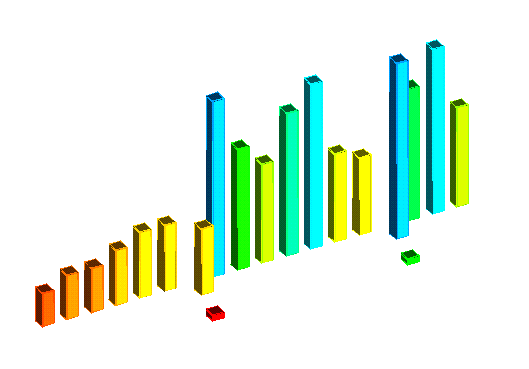
\includegraphics[width=0.6\textwidth]{pavaneSfondoAzzurro.png}
		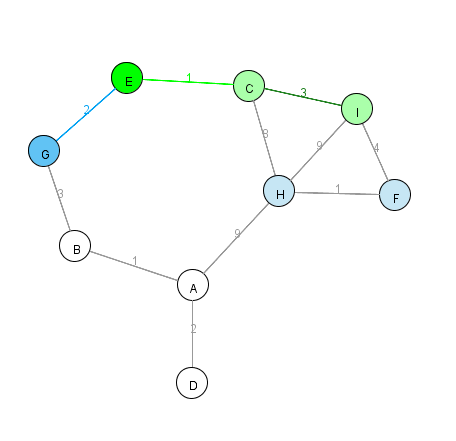
\includegraphics[width=0.4\textwidth]{grafo.png}
	\end{frame}
	
	%frame 3
	\begin{frame}
		\frametitle{Visualizzazione di Algoritmi}
		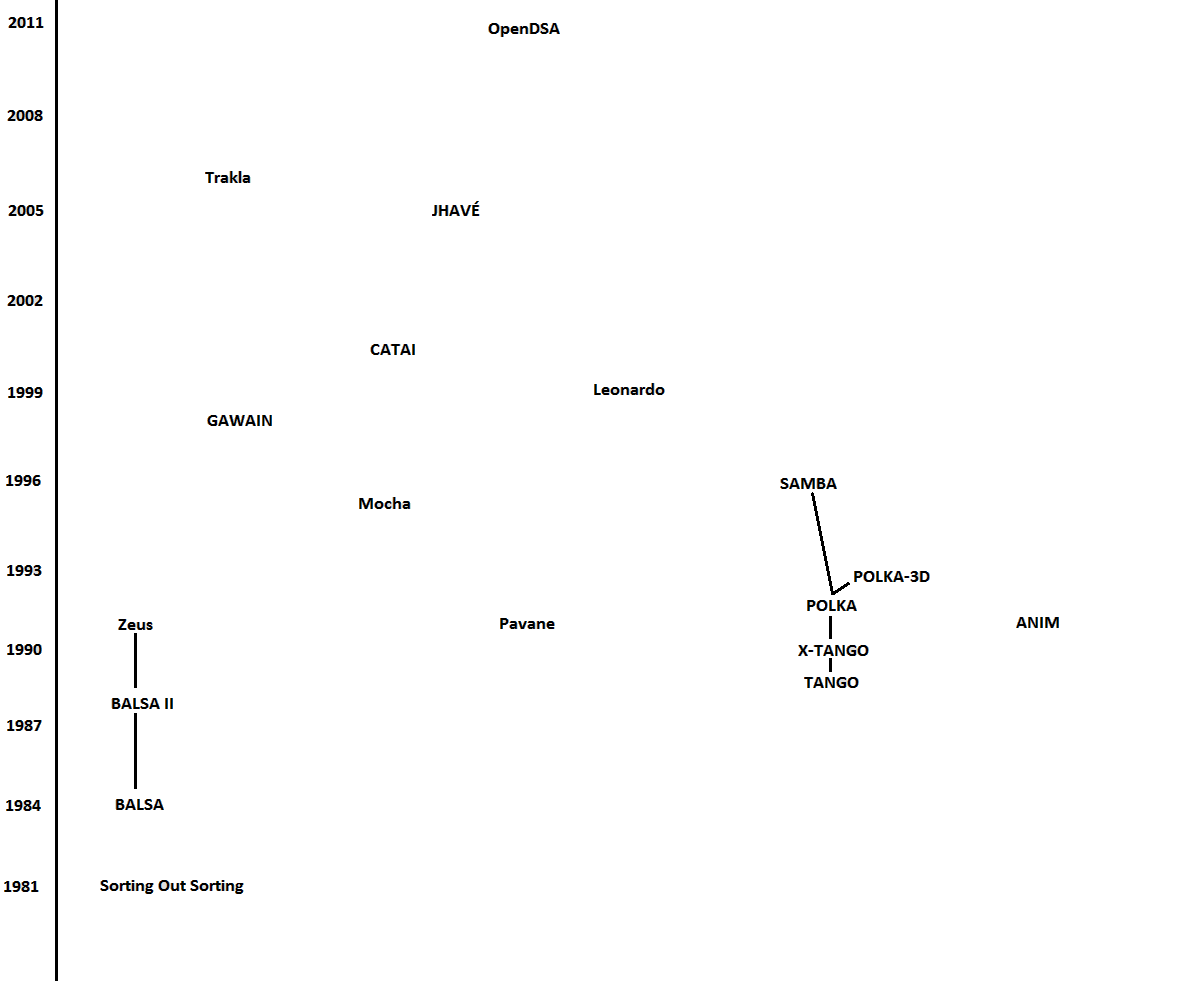
\includegraphics[height=0.9\textheight]{schema.png}
	\end{frame}

	%frame 4 new
	\begin{frame}
		\frametitle{HTML5 \& Canvas}
		\begin{alertblock}{HTML5: il nuovo standard per il Web}
			\begin{itemize}
				\item Gestione di applicazioni multimediali.
				\item Creazione in tempo reale di grafica 2D e 3D.
			\end{itemize}
		\end{alertblock}
		Canvas (dall'inglese, \textit{tela}) � l'area di disegno supportata nativamente da HTML5.
		\begin{itemize}
			\item Creazione e gestione di grafica bitmap 2D in tempo reale.
			\item Programmazione grafica in JavaScript.
			\item Costo computazionale e occupazione di memoria molto bassi.
		\end{itemize}
		\begin{center}
			\begin{tikzpicture}
				\node[
					draw=none,
					blur shadow={shadow blur steps=10, shadow xshift=.8ex, shadow yshift=-.8ex}
				] at (0,0) {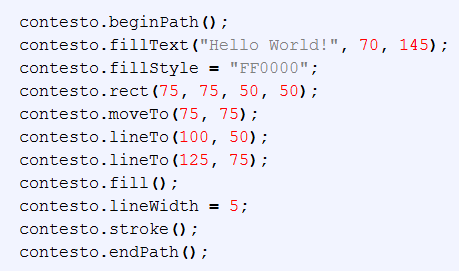
\includegraphics[scale=0.3]{codice.png}};
				\node[
					draw,
					fill=white,
					blur shadow={shadow blur steps=10, shadow xshift=.8ex, shadow yshift=-.8ex},
					rounded corners
				] at (1.2,-0.5) {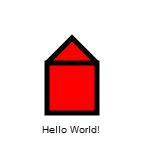
\includegraphics[scale=0.3]{esempio3.png}};
			\end{tikzpicture}
		\end{center}
	\end{frame}

%	%frame 4
%	\begin{frame}
%		\frametitle{HTML5}
%		HTML5 nasce da una scissione del W3C (\textit{World Wide Web Consortium}) avvenuta nel 2004.
%		\begin{itemize}
%			\item Gestione di applicazioni multimediali.
%			\item Creazione in tempo reale di grafica 2D e 3D.
%			\item Gestione degli errori.
%			\item Aggiunti nuovi tag ed eliminati tag deprecati.
%			\item Gestione di formule matematiche.
%		\end{itemize}
%		\begin{center}
%			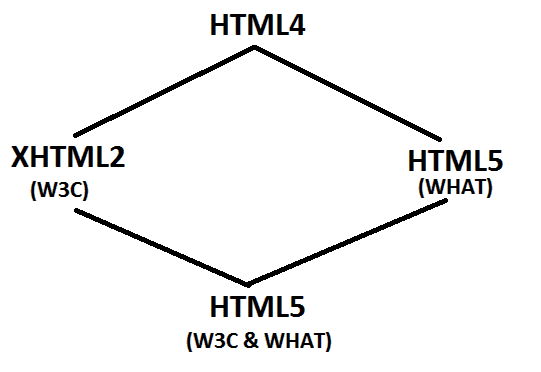
\includegraphics[scale=0.5]{html5.png}
%		\end{center}
%	\end{frame}
%	
%	%frame 5
%	\begin{frame}
%		\frametitle{Canvas}
%		Canvas (dall'inglese, \textit{tela}) � l'area di disegno supportata nativamente da HTML5.
%		\begin{itemize}
%			\item Creazione e gestione di grafica bitmap 2D in tempo reale.
%			\item Programmazione grafica in JavaScript.
%			\item Costo computazionale e occupazione di memoria molto bassi.
%		\end{itemize}
%		\begin{center}
%			\begin{tikzpicture}
%				\node[
%					draw=none,
%					blur shadow={shadow blur steps=10, shadow xshift=.8ex, shadow yshift=-.8ex}
%				] at (0,0) {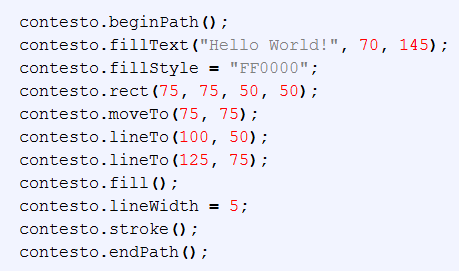
\includegraphics[scale=0.5]{codice.png}};
%				\node[
%					draw,
%					fill=white,
%					blur shadow={shadow blur steps=10, shadow xshift=.8ex, shadow yshift=-.8ex},
%					rounded corners
%				] at (2,-1) {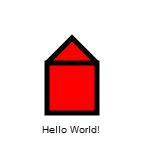
\includegraphics[scale=0.3]{esempio3.png}};
%			\end{tikzpicture}
%		\end{center}
%	\end{frame}
	
	%frame 5
	\begin{frame}
		\frametitle{AlViE}
		AlViE (\textit{Algorithm Visualization Environment}) � un ambiente di visualizzazione di algoritmi scritto in Java.
		\begin{itemize}
			\item Visualizzazioni 2D a colori.
			\item Navigazione attraverso gli step (o passi) dell'algoritmo.
			\item Possibilit� di implementare i propri algoritmi in Java per la visualizzazione su AlViE.
			\item Possibilit� di salvare e ricaricare in un secondo momento le visualizzazioni prodotte (salvate su file XML).
			\item Alto grado di personalizzazione della visualizzazione.
			\item Pseudocodice e messaggio per ogni step di visualizzazione.
			\item Selezione di diversi tipi di zoom.
		\end{itemize}
	\end{frame}
	
	%frame 6
	\begin{frame}
		\frametitle{AlViE}
		\begin{center}
			\begin{tikzpicture}
				\node[
					draw=none,
					blur shadow={shadow blur steps=10, shadow xshift=.8ex, shadow yshift=-.8ex}
				] at (0,0) {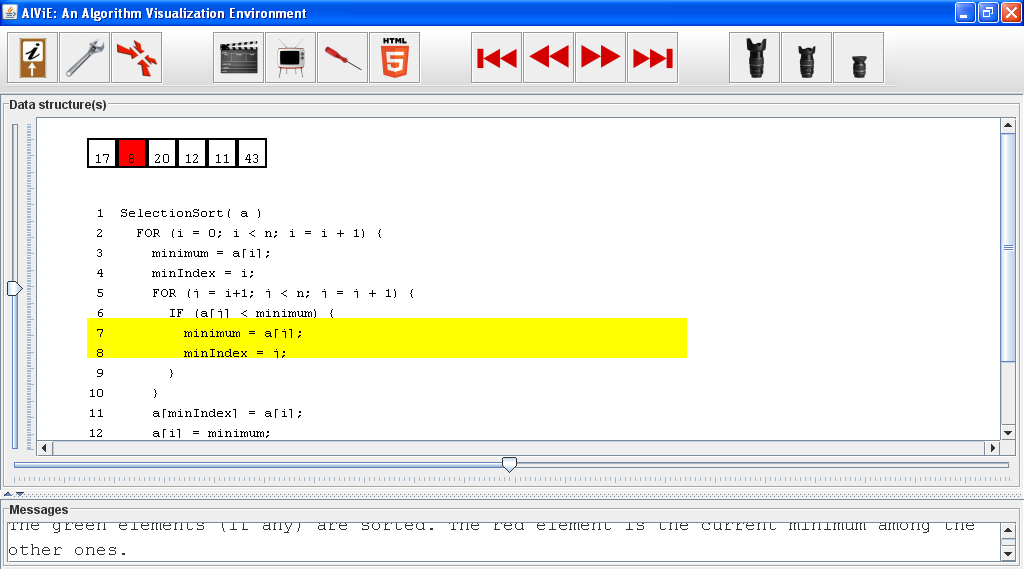
\includegraphics[scale=0.3]{alvie.png}};
			\end{tikzpicture}
		\end{center}
	\end{frame}
	
	%frame 7
	\begin{frame}
		\frametitle{AlViE 4}
		Le principali novit� introdotte con la quarta versione di AlViE sono:
		\begin{itemize}
			\item esportazione delle visualizzazioni in pagine HTML;
			\item un editor di strutture dati.
		\end{itemize}
		\begin{center}
			\begin{tikzpicture}
				\node[
					draw=none,
					blur shadow={shadow blur steps=10, shadow xshift=.8ex, shadow yshift=-.8ex}
				] at (0,0) {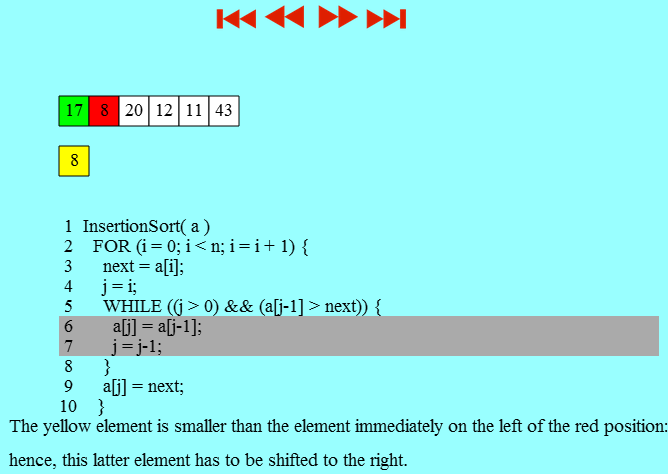
\includegraphics[scale=0.3]{alvieHTML5.png}};
				\node[
					draw=none,
					blur shadow={shadow blur steps=10, shadow xshift=.8ex, shadow yshift=-.8ex},
					rounded corners
				] at (2,-1) {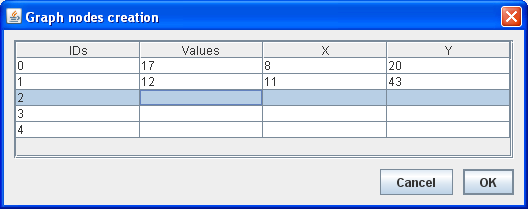
\includegraphics[scale=0.3]{inputEditor.png}};
			\end{tikzpicture}
		\end{center}
	\end{frame}
	
	%frame 8
	\begin{frame}
		\frametitle{Compilatore XML-HTML5}
		\begin{center}
			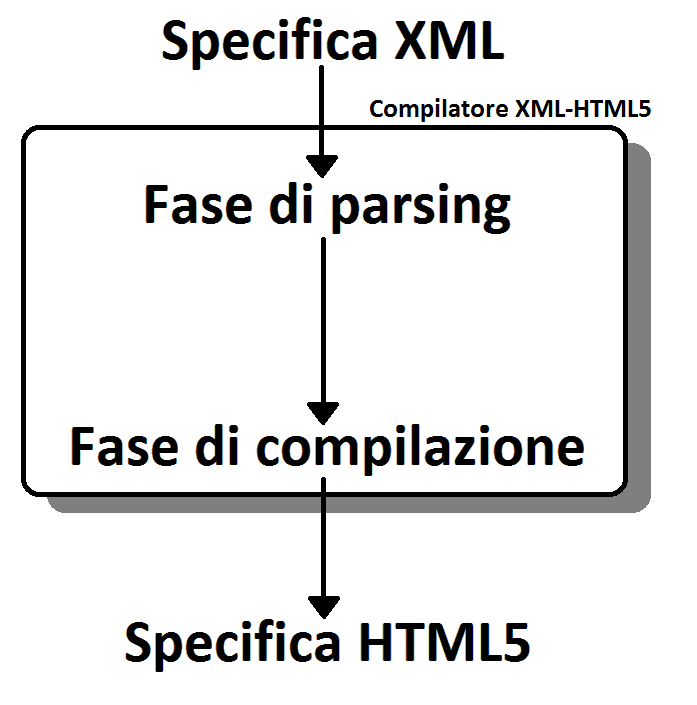
\includegraphics[height=0.8\textheight]{parsingCompilazione.png}
		\end{center}
	\end{frame}
	
	%frame 9
	\begin{frame}
		\frametitle{Parsing}
		\begin{center}
			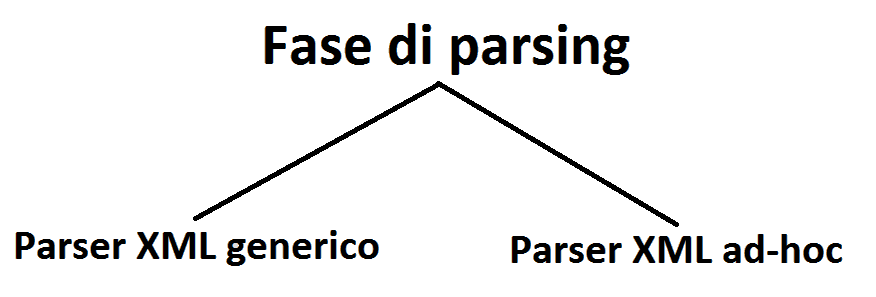
\includegraphics[scale=0.5]{parsing.png}
		\end{center}
		\begin{center}
			\begin{tabular}{|c|c|c|}
				\hline
				\textbf{Algoritmo} & \textbf{Parser ad-hoc} & \textbf{Digester}\\
				\hline
				LCS & 2.64 s & 10.4 s\\
				\hline
				Dijkstra & 0.92 s & 2.75 s\\
				\hline
				QuickSort & 1.04 s & 1.51 s\\
				\hline
				Commesso viaggiatore & 0.46 s & 1.65 s\\
				\hline
			\end{tabular}
		\end{center}
		\tiny Test eseguiti su un calcolatore Netbook Packard Bell, CPU Intel Atom N280 @1.66 GHz, 1GB di memoria RAM, Sistema Operativo Windows XP Home Edition SP3.
	\end{frame}
	
	%frame 10
	\begin{frame}
		\frametitle{Compilazione}
		\begin{center}
			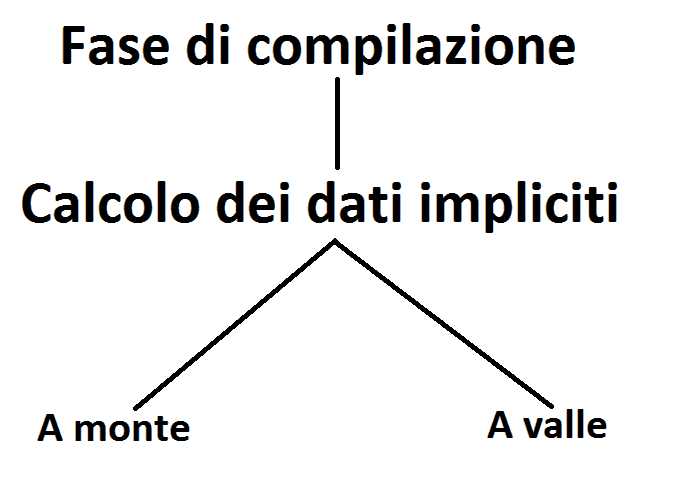
\includegraphics[scale=0.4]{compilazione.png}
		\end{center}
		Durante la fase di compilazione devono essere calcolati i \underline{dati impliciti} degli oggetti grafici:
		\begin{itemize}
			\item \textbf{calcolo a monte:} il compilatore e la pagina vengono appesantiti, il browser viene alleggerito;
			\item \textbf{calcolo a valle:} il compilatore e la pagina vengono alleggeriti, il browser viene appesantito.
		\end{itemize}
	\end{frame}
	
	%frame 11
	\begin{frame}
		\frametitle{Compilazione}
		\framesubtitle{Schema generale}
		\begin{center}
			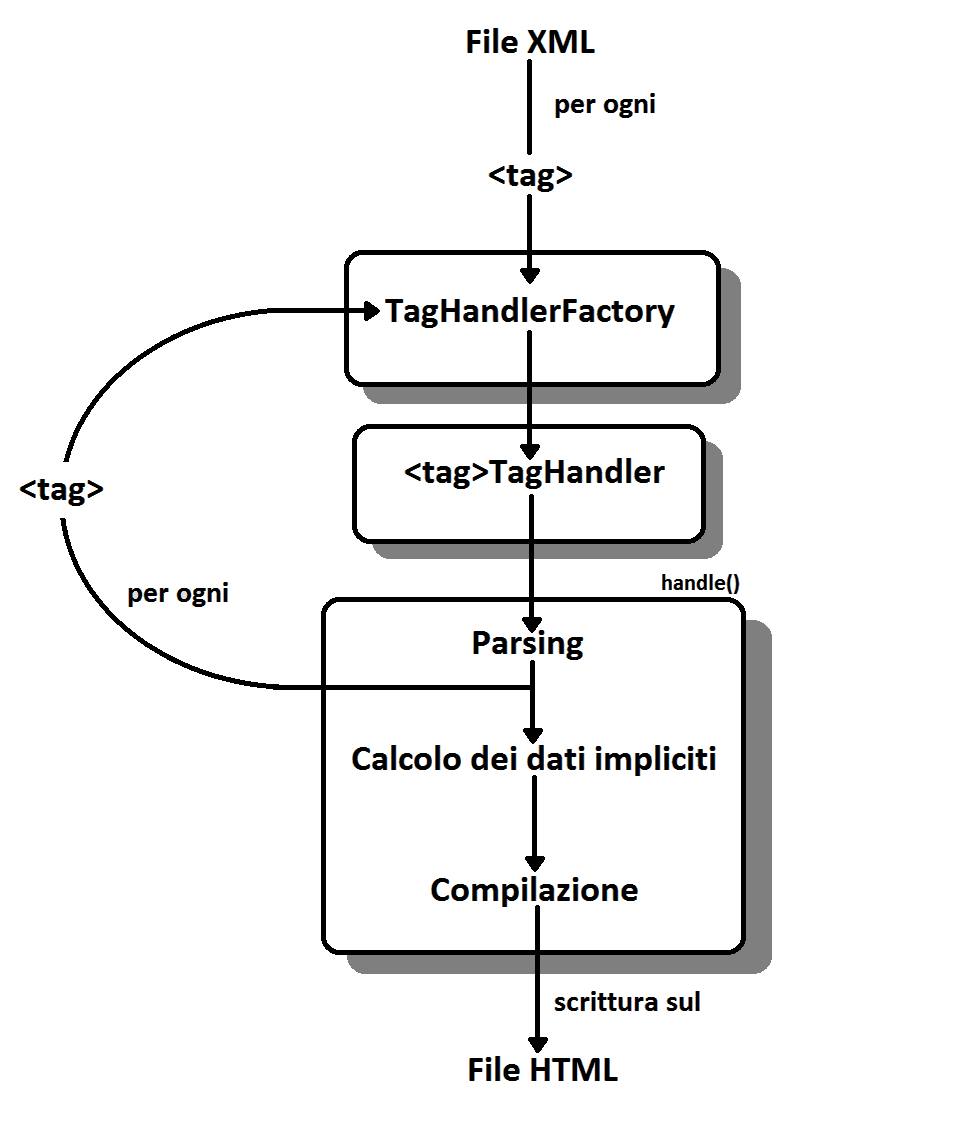
\includegraphics[height=0.8\textheight]{schemaCompilazione.png}
		\end{center}
	\end{frame}
	
	%frame 12
	\begin{frame}
		\frametitle{Un esempio}
		\framesubtitle{Gestione di un array}
		\begin{center}
			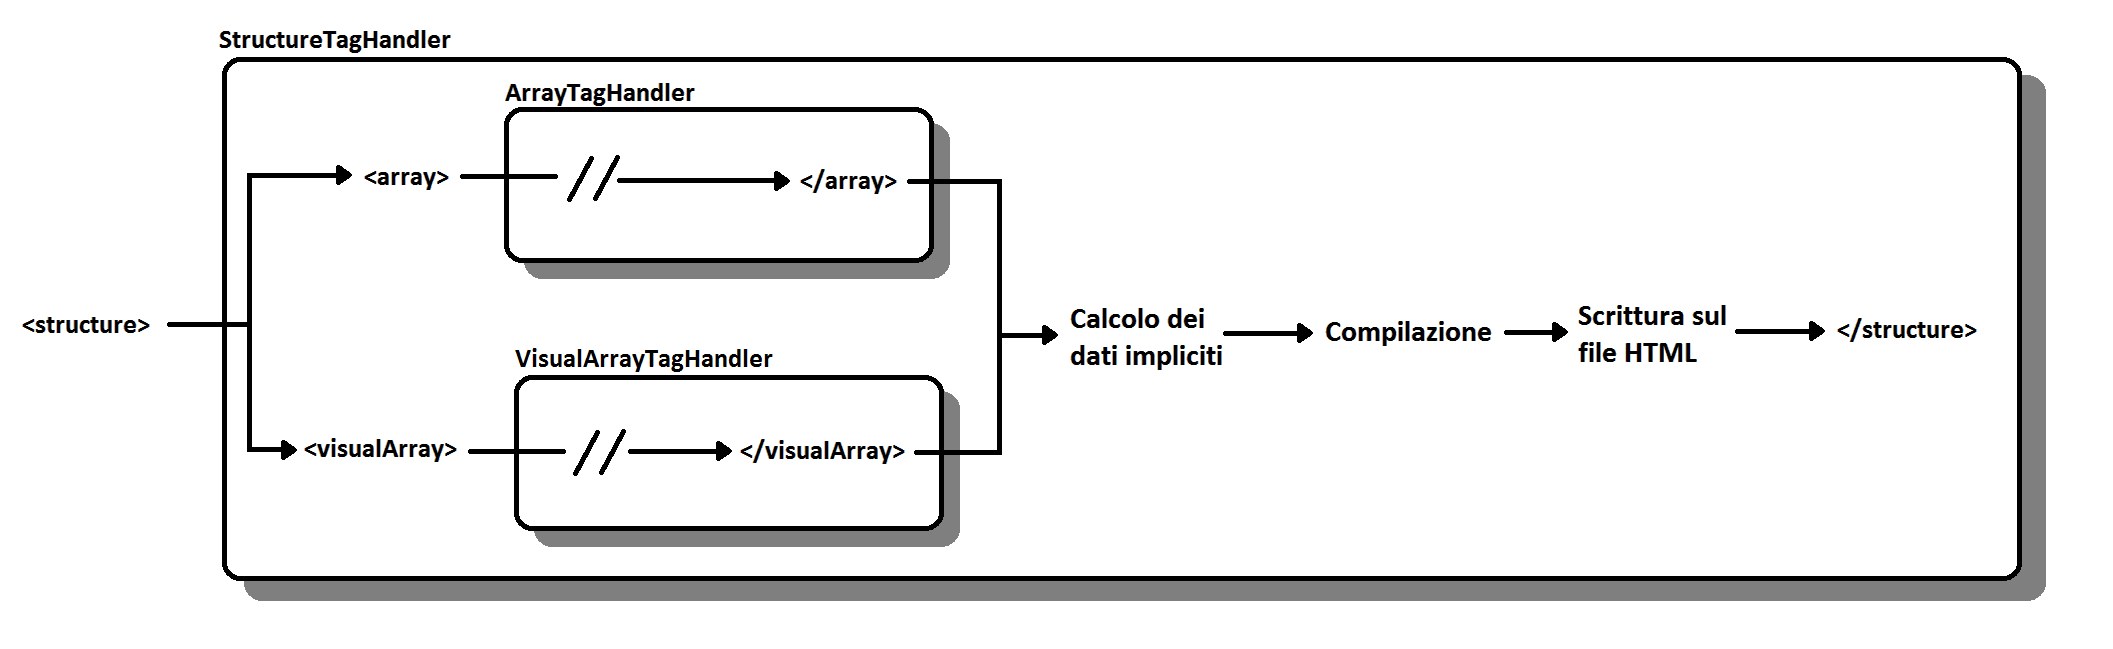
\includegraphics[width=\textwidth]{schemaArray.png}
		\end{center}
		La specifica di ogni struttura dati � suddivisa in due parti:
		\begin{itemize}
			\item una parte contenente le informazioni che definiscono la struttura dati;
			\item una parte che contenente le specifiche grafiche necessarie per disegnare la struttura.
		\end{itemize}
	\end{frame}
	
	%frame 13
	\begin{frame}
		\frametitle{Un esempio}
		\framesubtitle{Nel dettaglio: ArrayTagHandler}
		\begin{center}
			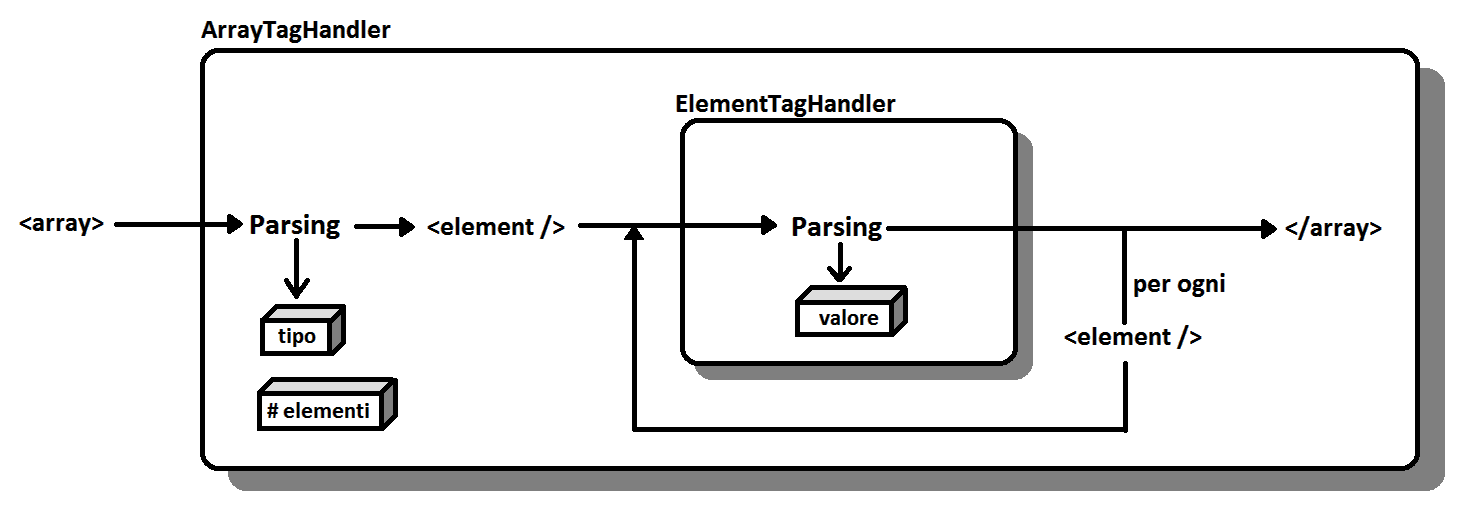
\includegraphics[width=\textwidth]{schemaArrayTag.png}
		\end{center}
	\end{frame}
	
\end{document}